\chapterauthor{Karl Thyssen}
Here we will discuss the results we saw for the various approaches we attempted.

As previously mentioned we experimented with a $\gamma$ value of $1.0$ and $0.9$ after which we continued other variations at $\gamma = 0.9$.
Other variations include:
\begin{itemize}
	\item $\gamma = 1.0$:
	\begin{itemize}
		\item Generation 0 data generated from 4 $\code{simple\_agents}$
		\begin{itemize}
			\item Additionally train MLB
		\end{itemize}
	\end{itemize}
	\item $\gamma = 0.9$:
	\begin{itemize}
		\item Generation 0 data generated from 4 $\code{simple\_agents}$:
		\begin{itemize}
			\item self-train until agents begin to regularly interact with each other
			\item self-train
			\item state vector reduced to 180 elements
		\end{itemize}
	\end{itemize}
\end{itemize}

%Discuss reasons behind initial approach - also mlp regressor (slow to fit so less data)
\subsection{The initial approach}
\chapterauthor{Karl Thyssen}
Having decided on the random forest regressors as the medium for storing our Q, and knowing the random forest has the ability to determine feature importances and weightings itself we decided to throw every feature we could think of at it as described in \ref{State_rep_1}. We initially also chose a $\gamma$ value of $1.0$ for simplicity in testing and began to train an agent. In \cite{paper} the agent trains for 10000 episodes per generation and begins to show a large improvement between generations $0$ and $20$, however that agent is trained using a neural network so we expected a longer wait before seeing such spikes in performance. This is due to the erratic nature of the predictions made by the forests in relation to the MLP we tested.

Out of interest we also tested the same set-up using an MLP regressor, however unlike the forest, the impact of using any and all features was an exorbitant time required for the fitting after each generation, often longer than the data generation itself.

The time required to generate data for and fit each generation was between $4800$ and $10000$ seconds for the random forest. This time required is clearly dependent not only on hardware and thinking time but also the number of steps the agent takes per episode which was, unfortunately, consistently short.

\begin{figure}[!h]
\centering
	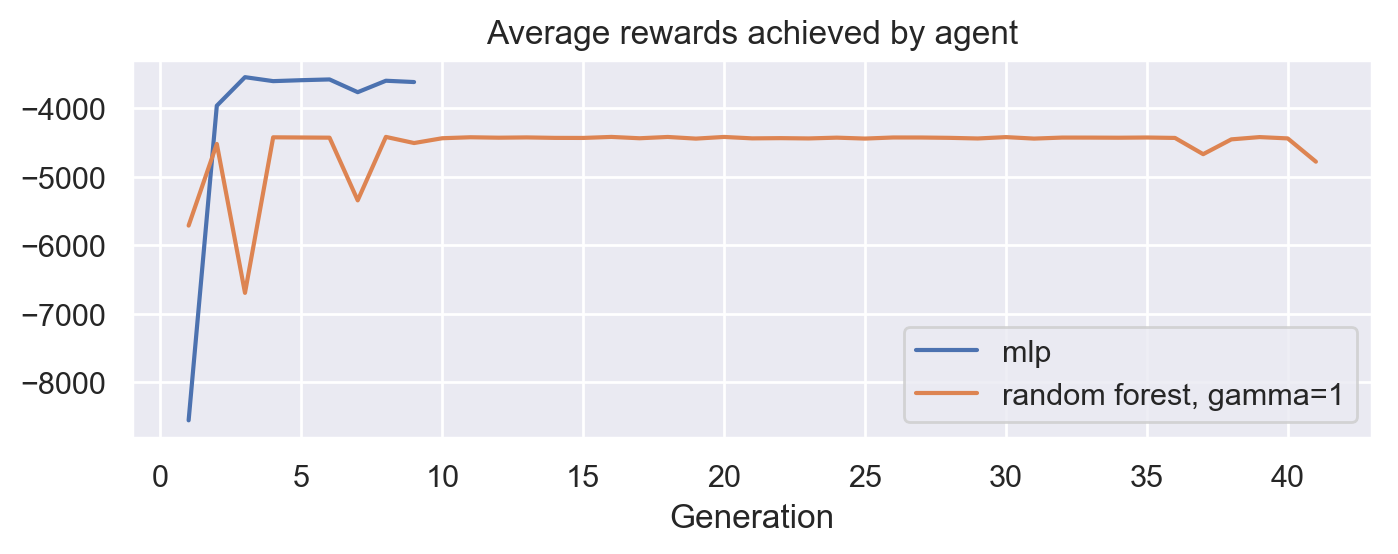
\includegraphics[width=\linewidth]{images/mlp_vs_forest_gamma_1.png}
	\caption{\textit{Here we see the performance of 40 generations trained with the random forest and 8 generations using the MLP. We chose not to train the MLP further as the time constraints were too severe and we were not seeing any improvement.}}
	\label{mlp_vs_forest_gamma_1.0}
\end{figure}

After these results we assessed potential reasons for such a static reward graph, that is to say a plateau in the rewards attained. To improve the quality of the next agent we looked at the following aspects of our learning process:
\begin{itemize}
	\item Firstly we looked at the exploration policy which originally effectively lead the agent to choose a non-$\pi$ based action every $4$ moves with $\epsilon=0.25$. We realised this would probabilistically cap the number of moves the agent would do before placing a bomb in a possibly precarious situation with $\#Action=6$ at $\frac{6}{0.25}=24$ moves. We chose to edit the exploration structure to follow what we discuss in \ref{explo}, to ensure exploration effectively occurs in $\epsilon*100\%$ of games rather than in every game, effectively increasing exploitation. Although exploitation leads to plateaus in general once the agent has fully exploited a particular policy it is using, we hope it explores often enough to prevent this and see more danger in the agent never learning how to play further than $24$ moves. 
	\item Secondly we looked at our rewards which originally offered $100$ points for a \state{coin\_found}, $10$ for an \state{invalid\_move}, $400$ for a kill and $-400$ for a death. We chose to exaggerate the rare but important events(coins, kills, death) to ensure that \textit{when} they occurred, they were noticed. We also harshly punished the \state{invalid\_move} as our first goal was to train an agent who knew how to manoeuvre through the map.
	\item Thirdly, after implementing a method to show the agents selected move, after a few generations we grew frustrated with the sheer quantity of \state{WAIT} actions the agent selected, and increased the punishment for the action to $-5$. This seemed to have the desired effect as 'wait until I die' runs were not seen again.
\end{itemize}

\subsection{Improving the learning process}
\chapterauthor{Karl Thyssen}
\subsubsection{Altering $\gamma$}
After seeing the poor results in terms of learning improvements of the random forest with $\gamma = 1.0$ we proceeded to introduce $\gamma = 0.9$. The hope was to allow the agent to differentiate between a good move and a poor move rather than between a good game and a bad game by isolating the individual moves more from later ones. However due to the delayed effect of the bombs and explosions the move itself \textbf{must} include rewards from later moves to some extent. While keeping all else equal the change in gamma value resulted in the agent surviving for noticeably longer than previously, the overall reward however doesn't seem to have benefited in the same way. This is despite an increase in the agents score, we assume this is due to the increased moves, costing the agent the points it receives for randomly picking up coins.

\begin{figure}[!h]
\centering
	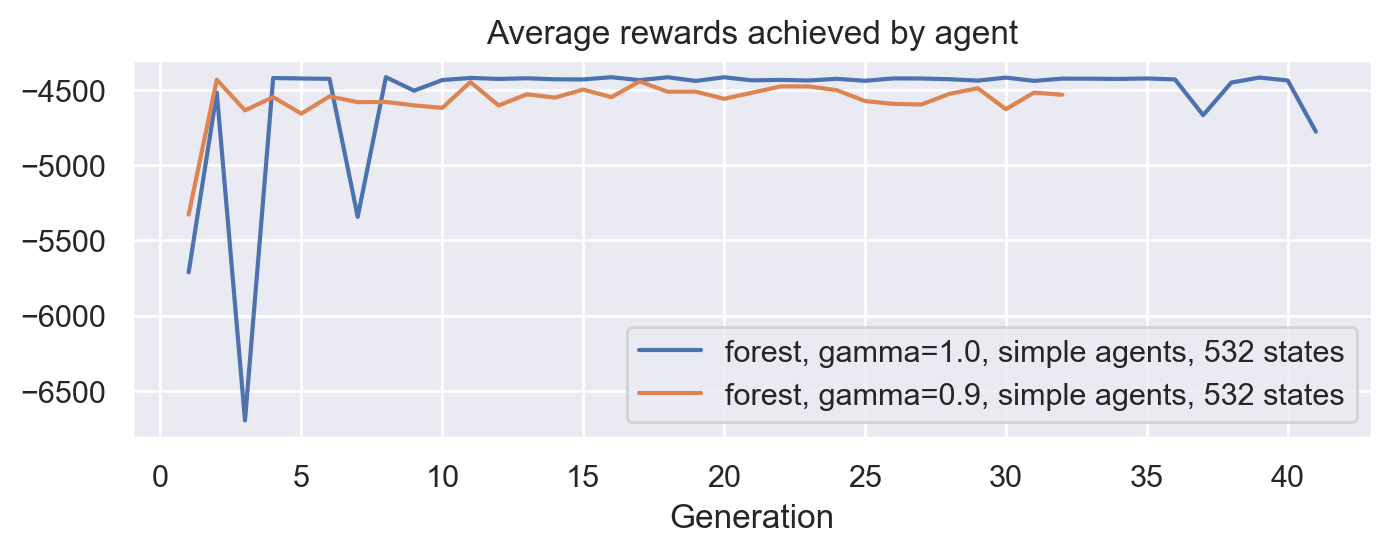
\includegraphics[width=\linewidth]{images/forest09_vs_forest1rew.png}
	\caption{\textit{Here we see the performance of the random forests trained with their respective gamma values, clearly there is no great difference in the rewards other, they both plateau within around 2 invalid move values of rewards of each-other. The relevant change is noticed in the rewards and survival graphs that follow.}}
	\label{forest09_vs_forest1rew}
\end{figure}

\begin{figure}[!h]
\centering
	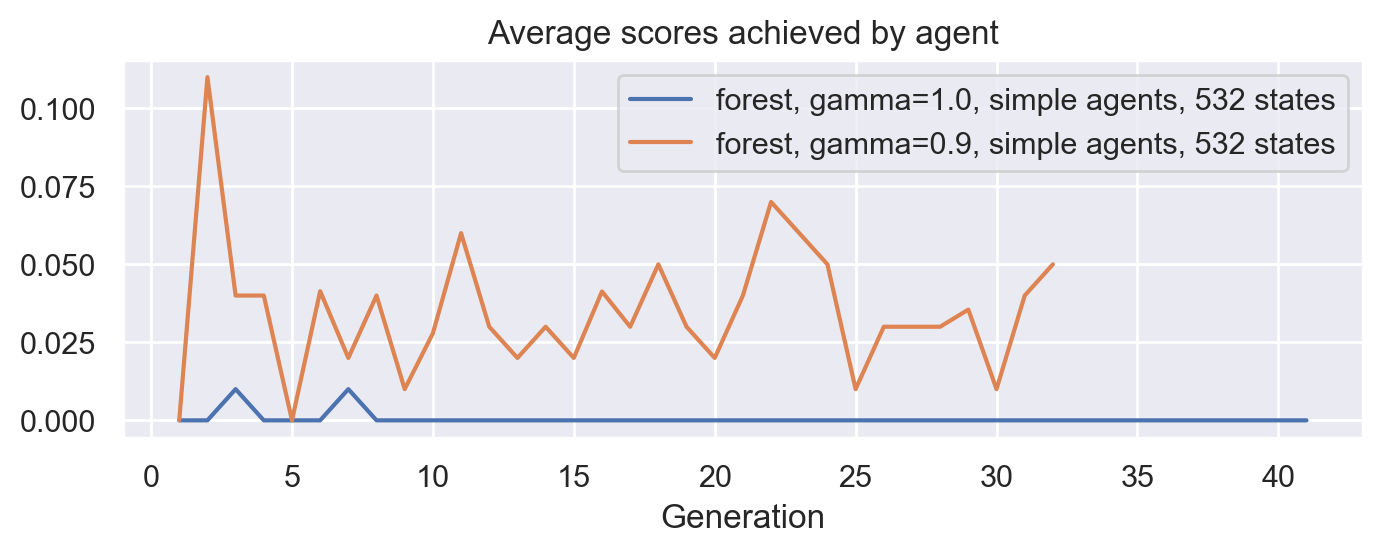
\includegraphics[width=\linewidth]{images/forest09_vs_forest1sco.png}
	\caption{\textit{Clearly the scores for the agent are not consistent throughout the generations, the primary difference being the fact that in 100 games the $\gamma = 0.9$ agent consistently collects the equivalent of 3 coins.}}
	\label{forest09_vs_forest1sco}
\end{figure}

\begin{figure}[!h]
\centering
	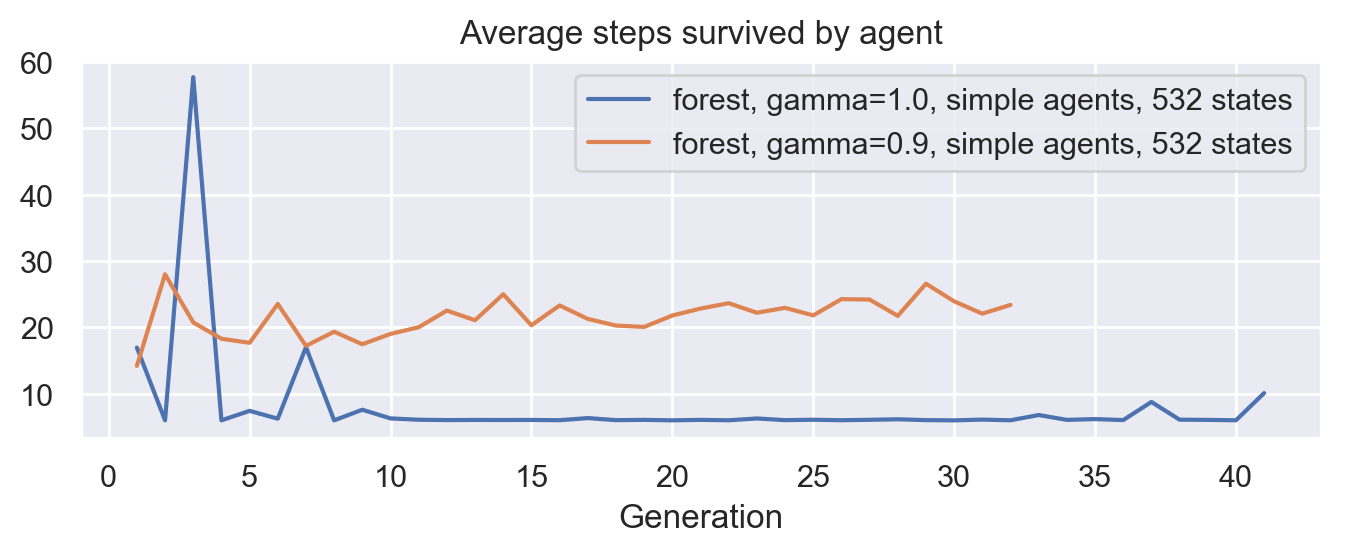
\includegraphics[width=\linewidth]{images/forest09_vs_forest1ste.png}
	\caption{\textit{While the agent with $\gamma = 1.0$ plateaus at 6 steps of survival, indicating his first action is to place a bomb and die to it after 5 steps, the other agent survives around 20 steps longer.}}
	\label{forest09_vs_forest1ste}
\end{figure}
\newpage
This indicates that some learning takes place as the agent no longer commits suicide early. Other points to support this are that most actions the agent performs must be valid, hence the discrepancy to the $\gamma = 1.0$ agent's baseline of only 200 points. Therefore the agent must have learnt how to make valid moves in the initial starting positions and must sometimes collect rewards(hence the points). This is corroborated purely qualitatively as we printed the agent's moves' validity and could observe a decrease in invalid moves after the first two generations. Unfortunately there doesn't seem to be a positive trend in any on these metrics to indicate improvement other than potentially a very small gain in survival steps.

\subsection{streamlining the state vector}
Our initial approach having been the 'the more the merrier' variant we decided to assess look at the state vector again to remove redundancies. There are many alternative methods to present the state vector, which we will discuss later, wishing to stay close to our original schematic we selected however to simplify our original rather than changing it conceptually. Therefore we implemented the modified state vector in \ref{State_rep_2}.

\begin{figure}[!h]
\centering
	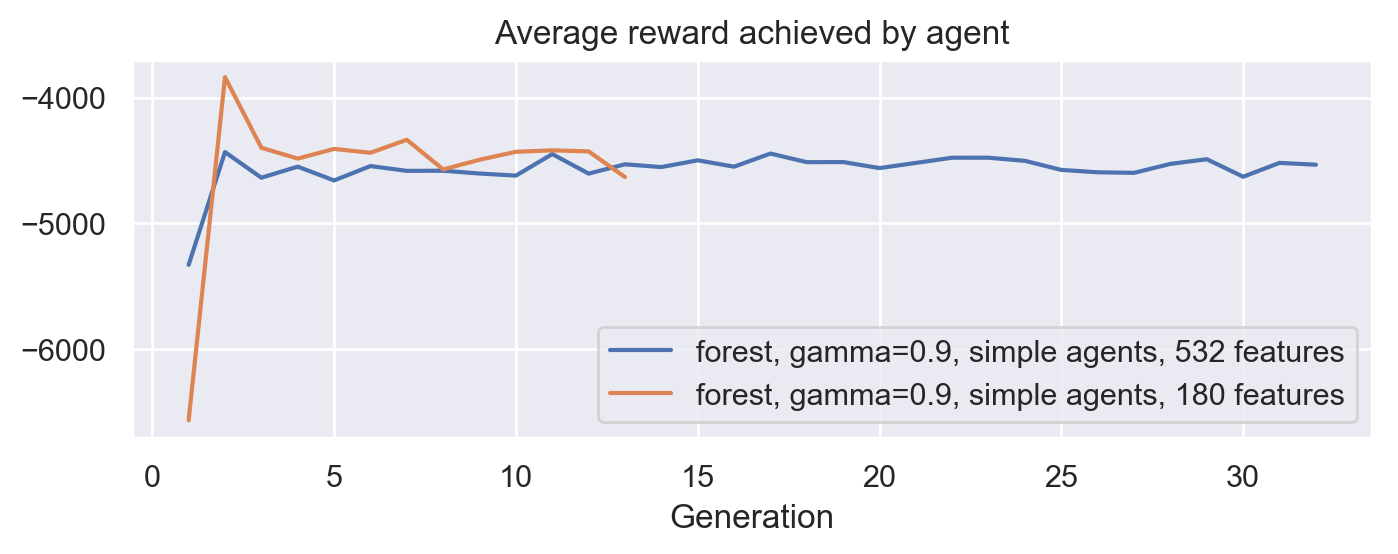
\includegraphics[width=\linewidth]{images/forest532_vs_forest180rew.png}
	\caption{\textit{As before, the reward graph is disappointing as it seems the agent does not learn to increase his reward any further despite clearly (as can be seen from the scores) not playing the game optimally.}}
	\label{forest532_vs_forest180rew}
\end{figure}

\begin{figure}[!h]
\centering
	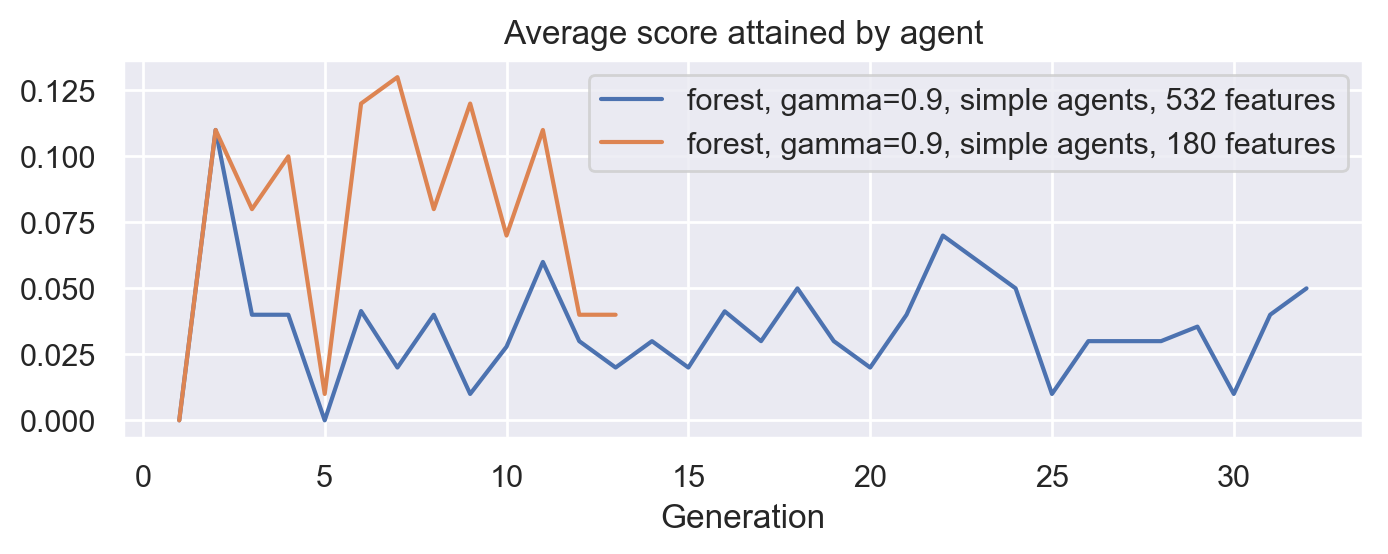
\includegraphics[width=\linewidth]{images/forest532_vs_forest180sco.png}
	\caption{\textit{The scores achieved for the agents trained in identical conditions other than their feature representation. Clearly the prevailing trend is for the scores of the simplified agent to be greater than those of the $532$ feature agent.}}
	\label{forest532_vs_forest180sco}
\end{figure}

\begin{figure}[!h]
\centering
	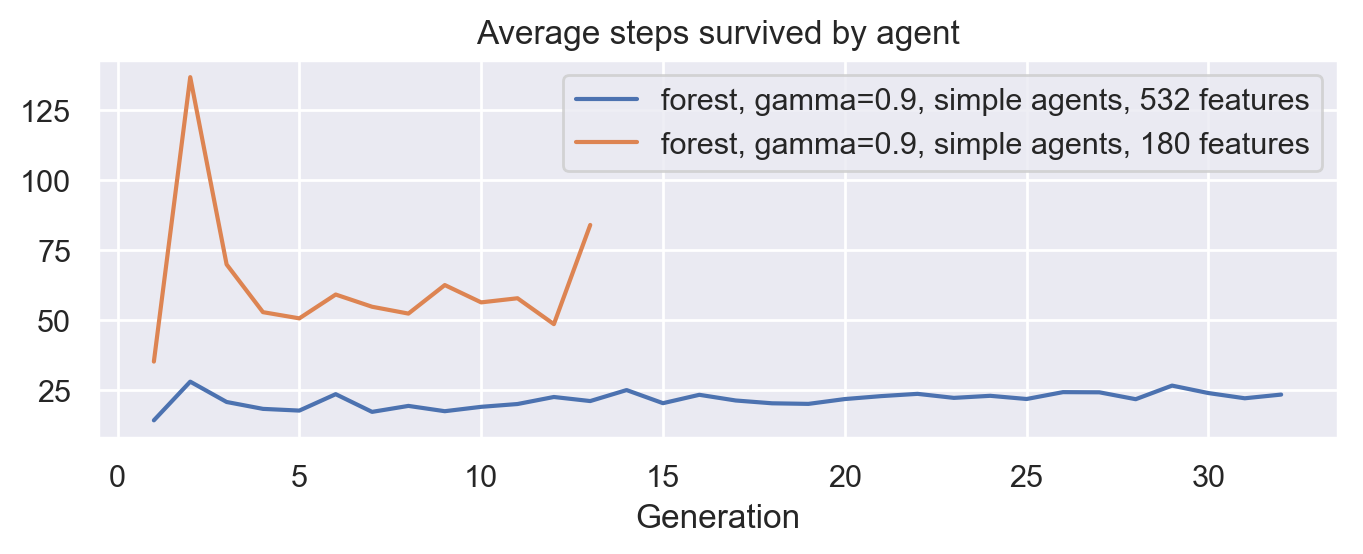
\includegraphics[width=\linewidth]{images/forest532_vs_forest180ste.png}
	\caption{\textit{The agent with its state vector consisting of $180$ features consistently survives longer than the one with the lager state vector.}}
	\label{forest532_vs_forest180ste}
\end{figure}

As we can see, the new agent does not achieve a greater average reward while consistently surviving longer and achieving a higher score. Overall a longer life while maintaining a close to equal reward implies a higher quality of moves as the negative reward obtained from moving at all, particularly if there are any invalid moves among this (as they are harshly punished) must be balanced out by for example destroying crates or obtaining coins.

At this point the next logical step, in hindsight, would have been an overhaul of the rewards, perhaps in some of the ways we explore later. However due to our earlier changes to the rewards and the fact we did not know how best to test for the best reward scheme we did not try variations on the rewards.

%show results of initial training
%random forest too erratic - as single steps can be fatal, inaccuracies can have drastic consequences
%let train for a long time as unclear when we should see results
%present variations
%discuss changes and possible solutions - even fewer features, other machine learning methods

\subsection{Outlook}
\chapterauthor{Hein-Erik Schnell, Karl Thyssen}
As discussed in the previous subsection, our agents are very unsuccessful. They mostly remain in their starting corner and more often than not they blow themselves up. It is therefore necessary to discuss alternative approaches to the task and how we could have improved our implemented approaches.\par

% More time, maybe they would have learned then -> more episodes per generation, more generations in general
% Exploration/Exploitation
% Much smaller state vector, no representation of the whole board
% Different initial settings of regressors
% Update regressors, not refit
% Different reward scheme, other gamma

As we see it, the topics to be discussed are mostly the sections above:
\begin{itemize}
	\item State representation
	\item Reward scheme
	\item Regressors
	\item Training procedure
	\item Exploration / Exploitation
\end{itemize}

\subsubsection{State Representation}
With what we saw so far, we have to assume that less features in the state vector lead to far less possible states and better performance of the agent. The $180$-features version of the state vector is already close to the smallest form of state vector possible if we want to represent the whole game board, which would be at least $176$ features ($176$ accessible cells). \par
A possible improvement would be a state vector which does not represent the whole game board. The simple agents, for example, only know the position of possible targets and whether they are in danger. With this in mind, we could create a state vector which gives only the informations relevant to the simple agents. Given that in most cases most of the game board is not relevant (especially at the beginning of an episode), this seems to be a quite reasonable approach. It would also help the agent to prioritize certain features, e.g. avoid explosions before collecting coins.

\subsubsection{Reward Scheme}
In the plots above, we see that achieved scores and rewards hardly correlate. In the ideal case, higher score means more rewards. Since this is not the case, we need to revisit our reward scheme and distribute much higher rewards for what actually scores. On the other hand, our agent died a lot which meant lots of penalties. But we don't get negative scores for dying. We don't really know which way is better and we would have tried both ways in order to find out.

\subsubsection{Regressors}
The regressors were the third crucial design choice. As hinted above, choosing a regressor which is very erratic (Random Forest Regressor) and one which we don't know much about (MLP-Regressor) left us somewhat dissatisfied. Still, they were the most practical choices to us.\par
For both regressors we used almost the default settings. Adjusting those settings accordingly to our task might have helped a lot. But in the case of the MLP-Regressor, we could only guess what effects the various parameters might have. \par

All in all, choosing a better suited regressor and adjusting its parameters properly are two of the most important tasks in order to improve our model.\par

One should also mention that, after each generation, we fitted a whole new Forest. One could try to adjust the former Forest towards the data, instead.

\subsubsection{Training procedure}
We mostly trained our model with $10000$ episodes per generation. In one case even for more than $40$ generations (i.e. $400000$ episodes). Since Reinforcement Learning sometimes requires long times before encountering a good policy, we could never know whether our agent is not able to learn properly (because of the points above) or if it just didn't have enough time. With almost no experience from prior projects or exercises concerning RL, we didn't know how to find out which is the case. Speaking of only the training procedure, having more episodes per generation and letting it run for more generations might always improve the results.

\subsubsection{Exploration / Exploitation}
As mentioned before, the agent tends to kill itself if \textit{exploration} is enabled because it is likely to take random actions shortly after having placed a bomb. In order to prevent this, one could lower the $\epsilon$ significantly. Apart from that, we think that \textit{exploration/exploitation} is of less importance in terms of improving the model. The bottleneck are the points mentioned in \textit{State Representation, Reward Scheme} and \textit{Regressors}. 

\subsection{Further Comments on the final project}
As already implied in several parts of the report, our greatest issue was the lack of knowledge and experience with Reinforcement Learning. Some exercises with feedback and sample solutions would have helped a lot. For the next time, I propose to divide the final project into subtasks which are then given to the students as the final one or two exercise sheets and let the final project be something like the final improvements to an already working environment and model.

